\documentclass[conference]{IEEEtran}
\IEEEoverridecommandlockouts
% The preceding line is only needed to identify funding in the first footnote. If that is unneeded, please comment it out.
\usepackage{cite}
\usepackage{amsmath,amssymb,amsfonts}
\usepackage{algorithmic}
\usepackage{graphicx}
\usepackage{textcomp}
\usepackage{xcolor}
\usepackage{multirow}
\usepackage{hyperref}
\def\BibTeX{{\rm B\kern-.05em{\sc i\kern-.025em b}\kern-.08em
    T\kern-.1667em\lower.7ex\hbox{E}\kern-.125emX}}
\begin{document}

\title{Fall Detection With Motion Tracking
}

\author{\IEEEauthorblockN{Jonathan Edmund Kusnadi}
\IEEEauthorblockA{\textit{Departemen Ilmu Komputer dan Elektronika} \\
\textit{Universitas Gadjah Mada}\\
Sleman, Indonesia \\
jonathan.edmund1202@mail.ugm.ac.id}
}

\maketitle

\begin{abstract}
    Deteksi jatuh merupakan area penelitian yang penting bagi masyarakat
    lanjut usia karena jatuh dapat menyebabkan cedera serius bahkan kematian. Dalam paper ini, kami mengusulkan sebuah program yang mengimplementasikan sistem deteksi jatuh untuk individu lanjut usia menggunakan penglihatan komputer.
\end{abstract}

\begin{IEEEkeywords}
penglihatan komputer, deteksi jatuh, visual tracking, masyarakat lanjut usia, keselamatan
\end{IEEEkeywords}

\section{Introduction}
Deteksi jatuh merupakan area penelitian penting bagi masyarakat lanjut usia karena jatuh dapat menyebabkan cedera serius bahkan kematian. Dalam paper ini, kami mengusulkan sebuah program yang mengimplementasikan sistem deteksi jatuh untuk individu lanjut usia menggunakan teknik tracking.

Selama beberapa dekade terakhir, banyak solusi yang telah dikembangkan untuk mendeteksi insiden jatuh secara otomatis. Teknologi pendeteksi jatuh biasanya mengandalkan tiga jenis perangkat: perangkat yang dapat dikenakan, sensor sekitar, dan kamera penglihatan. Perangkat yang dapat dikenakan bersifat mengganggu, dan perangkat tersebut harus dipasang dalam hubungan yang relatif dekat dengan subjek manusia. Sangat berat bagi para lansia untuk memakai perangkat fisik untuk jangka waktu yang lama. Perangkat berbasis suasana, seperti sensor audio dan getaran, telah digunakan dalam beberapa sistem pendeteksi jatuh. Perangkat berbasis suasana tidak terlalu mengganggu; namun, sifatnya yang kurang visibel membawa beberapa tantangan dalam membedakan jatuhnya benda mati dengan jatuhnya manusia. Pendekatan berbasis penglihatan memberikan solusi non-invasif dan andal untuk deteksi jatuh. Selain itu, kamera video telah banyak dipasang di berbagai bangunan umum dan fasilitas kesehatan untuk tujuan pengawasan. Ini adalah solusi berbiaya rendah untuk sistem deteksi jatuh yang praktis \cite{b1}.

Program yang diusulkan ini menggunakan algoritma deteksi manusia serta estimasi pose menggunakan model MoveNet untuk mengidentifikasi dan melacak individu dalam suatu ruangan. Kemudian, program menganalisis gerakan dari individu yang dilacak untuk menentukan apakah terjadi jatuh atau tidak. Tujuan dari program ini adalah memberikan sistem deteksi jatuh yang efektif dan akurat yang dapat dengan mudah diimplementasikan di berbagai lingkungan, termasuk panti jompo dan fasilitas perawatan lanjut usia. Sistem yang diusulkan juga dapat digunakan untuk memberikan peringatan secara real-time kepada pengasuh atau layanan darurat dalam kejadian jatuh. Efektivitas program yang diusulkan dievaluasi menggunakan dataset jatuh di dunia nyata, dan hasilnya menunjukkan bahwa sistem yang diusulkan mencapai tingkat akurasi dan ketahanan yang tinggi dalam mendeteksi jatuh. Paper ini menyajikan kontribusi berharga bagi bidang deteksi jatuh, dan program yang diusulkan berpotensi untuk meningkatkan keselamatan dan kesejahteraan individu lanjut usia.

\section{Methodology}

\subsection{Proposed Method}
Pendekatan yang diusulkan pada penelitian ini terdiri dari 4 langkah utama:
\begin{enumerate}
    \item Deteksi manusia dan estimasi pose menggunakan model MoveNet.
    \item Menghitung percepatan sudut pada antara hidung dan pinggul.
    \item Menghitung percepatan turun pada pusat masa.
    \item Jika kedua perhitungan melebihi batas tertentu, maka orang diklasifikasi jatuh.
\end{enumerate}

\subsection{Dataset}


\subsection{Object Detection and Pose Estimation}
Tahap pertama dari program yang diusulkan adalah mendeteksi manusia dan mengestimasi pose menggunakan model MoveNet. Movenet merupakan sebuah model Deep Learning yang dirancang untuk mengenali gerakan manusia dan memperkirakan pose tubuh dalam waktu nyata dengan menggunakan kamera. Model ini dikembangkan oleh Google Research pada tahun 2020 dan memanfaatkan arsitektur Convolutional Neural Network (CNN) untuk melakukan deteksi pose tubuh dan estimasi gerakan manusia.

\cite{b2} membahas mengenai rancangan dan arsitektur dari Movenet serta hasil evaluasi performa model pada beberapa dataset. Dalam paper tersebut dijelaskan bahwa Movenet dapat digunakan untuk mengenali gerakan manusia dengan akurasi yang tinggi serta dapat diintegrasikan pada aplikasi yang memerlukan estimasi pose tubuh dan gerakan manusia secara real-time.

Seperti pada Fig 1, sebuah citra atau gambar dari objek manusia akan dijadikan sebagai input untuk model Movenet. Kemudian, model akan menghasilkan output berupa titik-titik yang merepresentasikan pose tubuh manusia. Titik-titik tersebut dapat digunakan untuk mengidentifikasi pose tubuh manusia dan mengenali gerakan manusia. Letak titik-titik yang dapat merepresentasikan pose tubuh dapat dilihat pada Fig 2.

\begin{figure}[htbp]
    \centerline{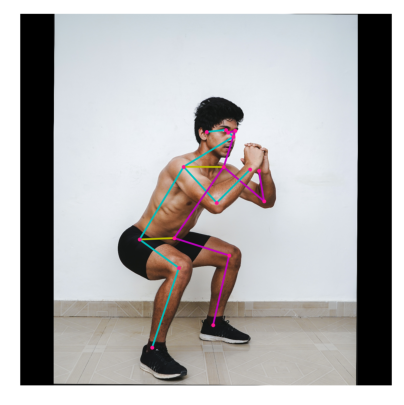
\includegraphics[width=0.5\textwidth]{figures/movenet1.png}}
    \caption{Estimasi Pose Menggunakan MoveNet.}
\end{figure}

\begin{figure}[htbp]
    \centerline{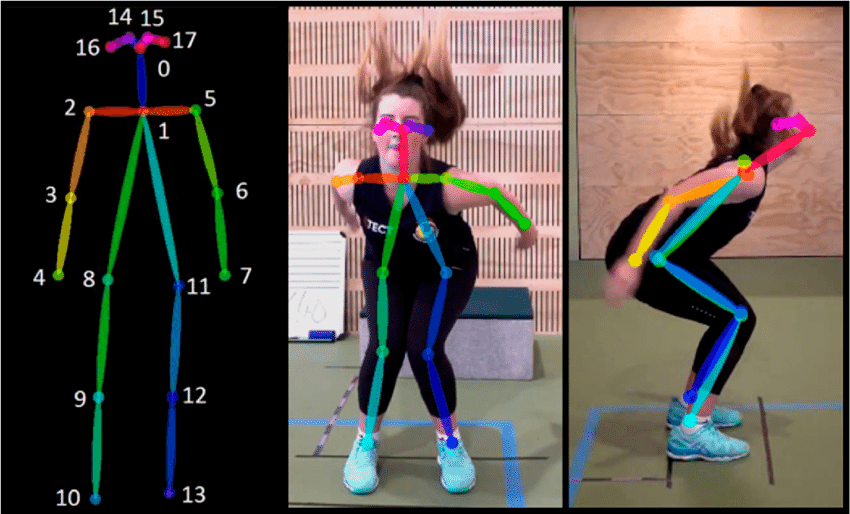
\includegraphics[width=0.5\textwidth]{figures/movenet2.png}}
    \caption{Letak Titik Pose.}
\end{figure}

\section{Fall Detection}
\subsection{Angular Acceleration}
Salah satu faktor yang digunakan dalam penelitian ini adalah percepatan sudut. Percepatan sudut merupakan perubahan kecepatan sudut dari suatu benda dalam waktu tertentu \cite{adachi2007fall}. Pada penelitian ini, jatuhnya seseorang akan menghasilkan perubahan sudut yang signifikan antara hidung dan pinggul \cite{liu2018fall}. Perubahan sudut ini terjadi dengan cepat, sehingga menghitung perpindahan percepatan sudut dapat menjadi faktor penting dalam mendeteksi jatuhnya seseorang. Percepatan sudut dapat dihitung dengan menggunakan persamaan \textit{finite second order backward difference} seperti yang dijelaskan oleh Adachi dan Wu \cite{adachi2007fall}.

\begin{equation}
f''(x)=\frac{f(x+h)-2f(x)+f(x-h)}{h^2}
\end{equation}

Rumus ini menghitung perubahan nilai sudut dari frame sebelumnya, dimana sudut dihitung dengan menggunakan titik yang terletak pada hidung dan pinggul \cite{han2019review}. Perhitungan nilai sudut tersebut dihitung dengan persamaan trigonometri seperti yang dijelaskan oleh Liu et al. \cite{liu2018fall}.

\begin{equation}
\theta=arctan(\frac{y_2-y_1}{x_2-x_1})
\end{equation}

Rumus ini menghitung nilai sudut dari dua titik yang terletak pada hidung dan pinggul. Nilai sudut tersebut kemudian digunakan untuk menghitung percepatan sudut dengan menggunakan persamaan (1).


\subsection{Center of Mass Descent}
Faktor kedua yang digunakan dalam penelitian ini adalah percepatan jatuh pada pusat massa. Percepatan jatuh pada pusat massa merupakan salah satu faktor yang digunakan dalam penelitian ini karena perpindahan pusat massa yang cepat secara vertikal dapat mengindikasi bahwa seseorang sedang jatuh. Perubahan posisi pusat massa ini terjadi dengan cepat, sehingga menghitung perpindahan percepatan turun dari pusat massa dapat menjadi faktor penting dalam mendeteksi jatuhnya seseorang. Percepatan jatuh pada pusat massa dapat dihitung dengan menggunakan persamaan finite second order backward difference seperti yang dijelaskan oleh Adachi dan Wu \cite{adachi2007fall}. Untuk menghitung percepatan tersebut diperlukan nilai posisi pusat massa yang didekati dengan nilai posisi pinggul pada frame sebelumnya.


\section{Results and Discussion}
Pada penelitian ini, digunakan perangkat komputasi GPU NVIDIA GeForce GTX 1650. Model MoveNet yang digunakan adalah versi \textit{lightning} karena menghasilkan deteksi serta estimasi pose pada objek manusia dengan baik.

\begin{figure}[htbp]
    \centerline{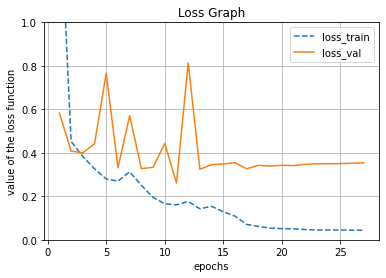
\includegraphics[width=0.5\textwidth]{figures/loss.png}}
    \caption{Grafik \textit{loss} dari model CNN}
\end{figure}

\begin{figure}[htbp]
    \centerline{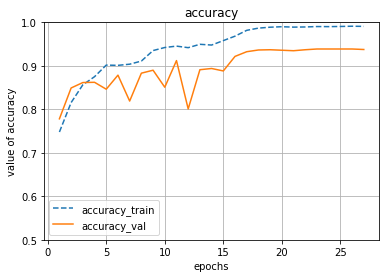
\includegraphics[width=0.5\textwidth]{figures/accuracy.png}}
    \caption{Grafik akurasi dari model CNN}
\end{figure}

Grafik \textit{loss} menunjukan bahwa model CNN yang diusulkan memiliki \textit{loss} yang semakin menurun seiring dengan bertambahnya epoch walaupun terjadi fluktuasi yang signifikan pada awal. Hal tersebut menunjukkan bahwa model CNN yang diusulkan semakin baik dalam melakukan klasifikasi gambar X-ray paru-paru.

Grafik akurasi menunjukkan bahwa model CNN yang diusulkan memiliki akurasi yang semakin meningkat seiring dengan bertambahnya epoch. Hal tersebut menunjukkan bahwa model CNN yang diusulkan semakin baik dalam melakukan klasifikasi gambar X-ray paru-paru.

Dari hasil pelatihan model CNN, didapatkan akurasi sebesar 94\% dan \textit{loss} sebesar 23\%. Hasil tersebut menunjukkan bahwa model CNN yang diusulkan memiliki performa yang baik dalam melakukan klasifikasi gambar.

\section{Conclusion}
Pada penelitian ini, model Convolutional Neural Network (CNN) terbukti dapat melakukan klasifikasi Covid-19 berdasarkan gambar X-ray paru-paru. Model CNN yang diusulkan memiliki akurasi sebesar 94\% dan \textit{loss} sebesar 23\%. Hasil tersebut menunjukkan bahwa model CNN yang diusulkan memiliki performa yang baik dalam melakukan klasifikasi gambar X-ray paru-paru. 

Untuk penelitian selanjutnya, dapat dilakukan penelitian dengan menggunakan dataset yang lebih besar dan beragam. Selain itu, dapat dilakukan penelitian dengan melakukan pengolahan citra seperti \textit{histogram equalization} beserta metode \textit{preprocessing} lainnya pada dataset. Untuk menghasilkan akurasi yang lebih tinggi, dapat dilakukan penelitian dengan menggunakan model CNN yang lebih kompleks seperti ResNet, DenseNet, dan EfficientNet. Dapat juga dilakukan penelitian dengan menggunakan \textit{transfer learning} untuk meningkatkan akurasi dari model CNN yang diusulkan.

\section{Additional Information}
File \textit{Google Colab} atau \textit{Jupyter Notebook} dapat diakses pada tautan berikut: \url{https://colab.research.google.com/drive/1dv7vCyRvFQis5hKDv8Sr2cJx3V8V1lo5}

\begin{thebibliography}{00}
\bibitem{b1} D. Ros and R. Dai, "A Flexible Fall Detection Framework Based on Object Detection and Motion Analysis," 2023 International Conference on Artificial Intelligence in Information and Communication (ICAIIC), Bali,Indonesia, 2023, pp. 063-068, doi: 10.1109/ICAIIC57133.2023.10066990.
\bibitem{b2} M. Andriluka et al., "Movenet: A Deep Learning Framework for Human Pose Estimation," in arXiv preprint arXiv:2103.11653 [cs.CV], Mar. 2021.
\bibitem{adachi2007fall} S. Adachi, Y. Abe, and M. Yachida, “Fall detection based on floor vibration measurement using a low-cost acceleration sensor,” in Proceedings of the 29th Annual International Conference of the IEEE Engineering in Medicine and Biology Society, 2007, pp. 2497–2500.
\bibitem{han2019review} Y. Han, H. Yoo, and D. Park, "A review on deep learning techniques for the recognition of human actions," International Journal of Control and Automation, vol. 12, no. 3, pp. 41-50, 2019.

\end{thebibliography}

\end{document}